% filepath: c:\Users\barte\source\repos\mm_projekt\raport.tex
\documentclass[12pt,a4paper]{article}
\usepackage[utf8]{inputenc}
\usepackage{polski}
\usepackage{amsmath}
\usepackage{graphicx}
\usepackage{hyperref}
\usepackage{geometry}
\geometry{margin=2.5cm}

\title{Raport z projektu w ramach przedmiotu \\ Modelowanie Matematyczne}
\author{Bartosz Chabros 198404 \and Beniamin Cymanowski 198067}
\date{\today}

\begin{document}

\maketitle

\section{Cel projektu}
Celem projektu było stworzenie aplikacji umożliwiającej symulację odpowiedzi układu dynamicznego z regulatorem PI na różne typy sygnałów wejściowych. Użytkownik może zmieniać parametry transmitancji, regulatora oraz sygnału wejściowego z poziomu interfejsu graficznego.

\section{Opis układu}
Układ składa się z transmitancji obiektu $G_p(s)$ oraz regulatora PI $G_c(s)$. Całość została zamknięta w pętli sprzężenia zwrotnego.

\subsection{Transmitancja obiektu}
\[
G_p(s) = \frac{a_1 s + a_0}{b_2 s^2 + b_1 s + b_0}
\]

\subsection{Regulator PI}
\[
G_c(s) = K_p + \frac{K_i}{s}
\]

\section{Interfejs użytkownika}
Aplikacja została napisana w języku Python z użyciem bibliotek PyQt6 oraz Matplotlib. Umożliwia ona:
\begin{itemize}
    \item Wprowadzanie parametrów transmitancji i regulatora,
    \item Wybór typu sygnału wejściowego (sinusoidalny, prostokątny, trójkątny),
    \item Ustawienie częstotliwości, fazy, czasu i kroku symulacji,
    \item Wizualizację sygnału wejściowego oraz odpowiedzi układu.
    \item Sprawdza stabilność układu i wyświetla o niej komunikaty w terminalu.
\end{itemize}

\section{Opis działania programu}
\begin{figure}[h!]
    \centering
    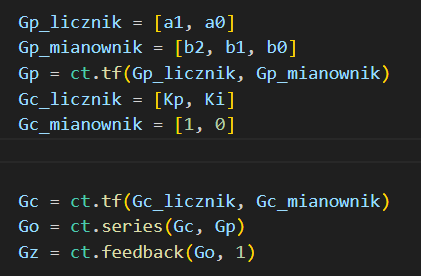
\includegraphics[width=0.8\textwidth]{wykres2.png}
    \caption{Po przekazaniu do funkcji run\_simulation są tworzone poszczególne transmitancje, są łączone szeregowo i zamykane w ujemnej pętli sprzężenia zwrotnego. W ten sposób otrzymujemy transmitancję całego układu.}
\end{figure}

\begin{figure}[h!]
    \centering
    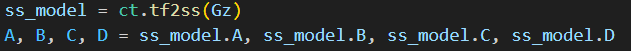
\includegraphics[width=0.8\textwidth]{model.png}
    \caption{Transmitancja całego układu jest następnie przekształcana na model stanowy.}
\end{figure}

\begin{figure}[h!]
    \centering
    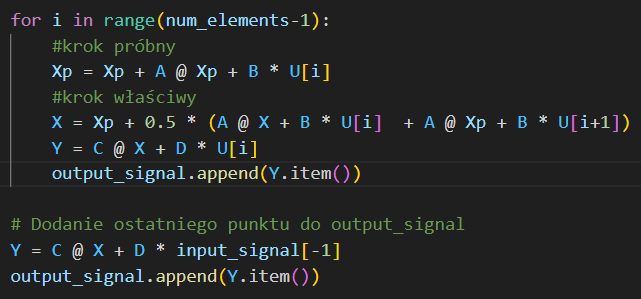
\includegraphics[width=0.8\textwidth]{pentla.png}
    \caption{Rozwiązywanie równań stanu jest realizowane przy pomocy metody Tustina.}
\end{figure}

\section{Przykładowe wyniki}
\begin{figure}[h!]
    \centering
    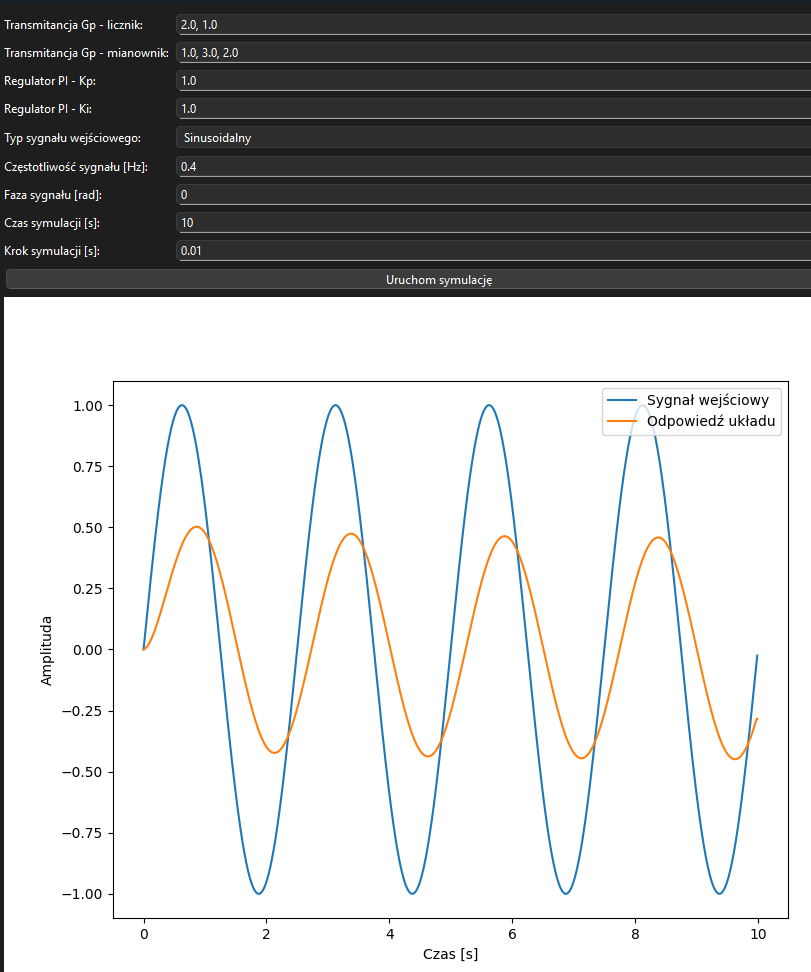
\includegraphics[width=0.8\textwidth]{wykres1.png}
    \caption{Przykładowa odpowiedź układu na sygnał sinusoidalny.}
\end{figure}

\begin{figure}[h!]
    \centering
    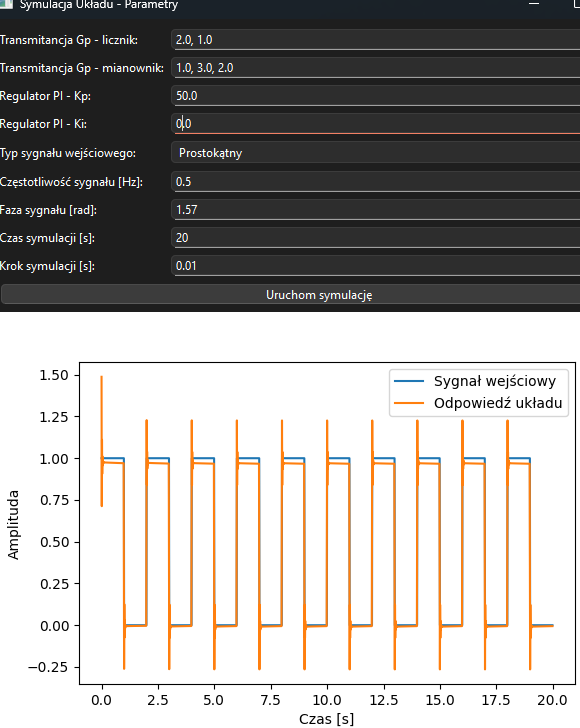
\includegraphics[width=0.8\textwidth]{wykres3.png}
    \caption{Przykładowa odpowiedź układu na sygnał prostokątny. Ilustracja przeregulowania.}
\end{figure}

\begin{figure}[h!]
    \centering
    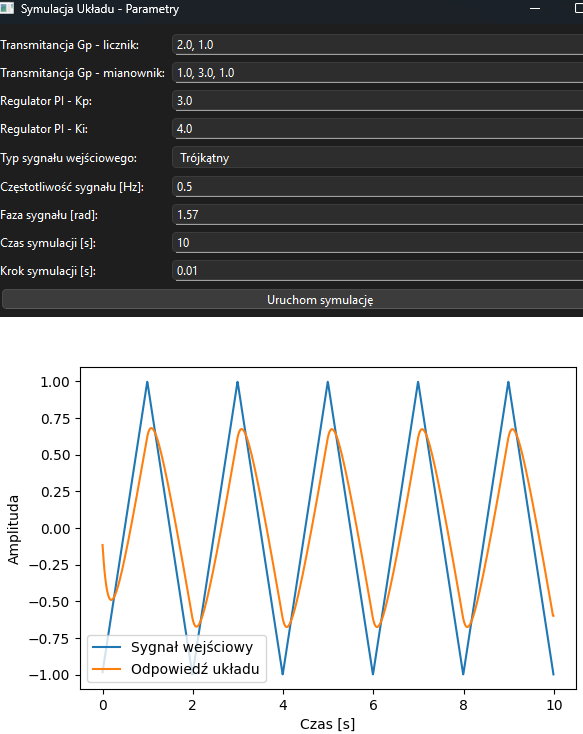
\includegraphics[width=0.8\textwidth]{wykres5.png}
    \caption{Przykładowa odpowiedź układu na sygnał trójkątny.}
\end{figure}

\section{Wnioski}
Wykorzystanie biblioteki Numpy oraz funkcji sawtooth oraz square z biblioteki SciPy pozwoliła na łatwą implementację sygnałów wejściowych.
Użycie biblioteki control pozwoliło na proste utworzenie transmitancji badanego układu oraz przekształcenie jej do modelu stanowego. W zasadzie jedyne ograniczenie w tworzeniu transmitancji obiektu i sterownika leży aktualnie w liczbie argumentów przyjmowanych przez funkcje run\_simulation (co można łatwo zmienić).
Dodatkowo fakt wykorzystania metody trapezów do rozwiązywania równań stanu pozwala na implementację innych sygnałów wejściowych, które posiadają miejsca nieciągłości(tak jak np. w przypadku sygnału prostokątnego) co byłoby problematyczne w przypadku zastosowania np, metody Taylora.
Zastosowanie modelu stanowego umożliwia również na łatwe rozszerzenie projektu o dodatkowe funkcjonalności jak np. dodanie elementów nieliniowych lub liczenie czy wykreślanie również sygnałów wewnętrznych układu(oczywiście wymagało by to przebudowy pętli realizującej symulacje tak aby liczyła stan każdego elementu układu).   



\end{document}